La clasificación, que implica la asignación de un objeto a una categoría específica, desempeña un papel fundamental tanto en la inteligencia humana como en la artificial. En este contexto, la clasificación abarca diversas tareas, que van desde determinar qué letra, palabra o imagen se ha presentado a nuestros sentidos, hasta reconocer caras, voces, clasificar correos electrónicos o calificar tareas.

El propósito subyacente de la clasificación es tomar una única observación, identificar y extraer características relevantes de la misma, y, en última instancia, ubicarla en una de las categorías discretas predefinidas.

\begin{definition}
Formalmente, definimos el problema de clasificación de texto, al escenario en que se tiene undocumento $d$ y un conjunto fijo de clases $C = \{c_1, c_2, \ldots, c_J\}$ y se requiere predecir un clase  $c \in C$ para $d$.
\end{definition}

Como se discutió en el Capítulo~\ref{cap_intro}, la construcción de clasificadores mediante reglas manuales no resulta ser un enfoque eficaz. Hoy en día la mayoría de las tareas de clasificación en PLN se abordan mediante enfoques de aprendizaje automático supervisado.

Formalmente, se parte de un conjunto fijo de clases $C = \{c_1, c_2, \ldots, c_J\}$ y un conjunto de entrenamiento compuesto por $m$ documentos que han sido etiquetados manualmente como
\[
(d_1, c_1), (d_2, c_2), \ldots, (d_m, c_m).
\]
A través de un proceso de entrenamiento, se desarrolla un clasificador que se define como una función $\gamma: d \to c$.

Diversos algoritmos de clasificación están disponibles para este propósito, como Naïve Bayes, Regresión logística, Redes neuronales, k-vecinos más cercanos, entre otros. En este capítulo, nos centraremos en el modelo Naïve Bayes. Este capítulo se basa en el material del curso de Daniel Jurafsky, al que se puede acceder a través del siguiente enlace\footnote{\url{https://web.stanford.edu/~jurafsky/slp3/4.pdf}}.

\section{Ejemplos de Problemas de Clasificación}
La clasificación de texto se puede aplicar a varias tareas, incluyendo:

\begin{itemize}
    \item Análisis de sentimientos
    \item Detección de spam
    \item Identificación de autoría
    \item Identificación de idioma
    \item Asignación de categorías, temas o géneros
\end{itemize}

Analicemos estos ejemplos en más detalle:

\begin{example}
Clasificación de spam. En este problema el objeto a clasificar es un correo eléctronico y las etiquetas posibles son SPAM y no SPAM. Las etiquetas se obtienen del mismo usuario que etiqueta los correos.

\begin{figure}[h]
    \centering
    
\includegraphics[scale = 0.35]{pics/spam.png}
    \caption{Ejemplo de Spam}
    \label{fig:chomsky}
\end{figure}


\end{example}




\begin{example}
Detección de Autoría. Un ejemplo histórico de detección de autoría se refiere a la autoría de los Ensayos Federalistas de la Constitución de EE. UU. En 1787, se escribieron ensayos anónimos para persuadir a Nueva York de ratificar la Constitución de EE. UU. La autoría de 12 de estos ensayos estuvo en disputa entre James Madison y Alexander Hamilton (Tabla~\ref{fig:autores}) hasta que en 1963, Mosteller y Wallace \cite{mosteller1963inference} utilizaron métodos bayesianos para identificar que Hamilton era el autor de los mismos.


\begin{table}[h]
    \centering
    \begin{tabular}{cc}
        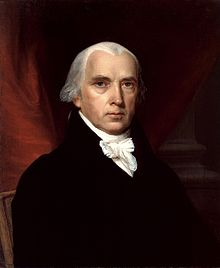
\includegraphics[height=0.3\textwidth]{pics/madison.png} & 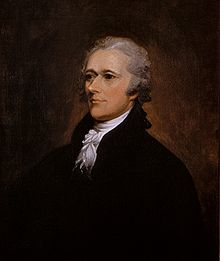
\includegraphics[height=0.3\textwidth]{pics/hamilton.png} \\
        James Madison & Alexander Hamilton \\
    \end{tabular}
    \caption{Autores candidatos a autoría.}
    \label{fig:autores}
\end{table}



\end{example}


\begin{example}
Clasificación por tópico. Aquí los ejemplos incluyen clasificar una noticia en una categoría temática (ej: deportes, política, economía) o etiquetar automáticamente un artículo en ciencias de la vida en una categoría del Medical Subject Headings (MeSH) como se ilustra en la Figura~\ref{fig:medarticle}.

\begin{figure}[h]
    \centering
    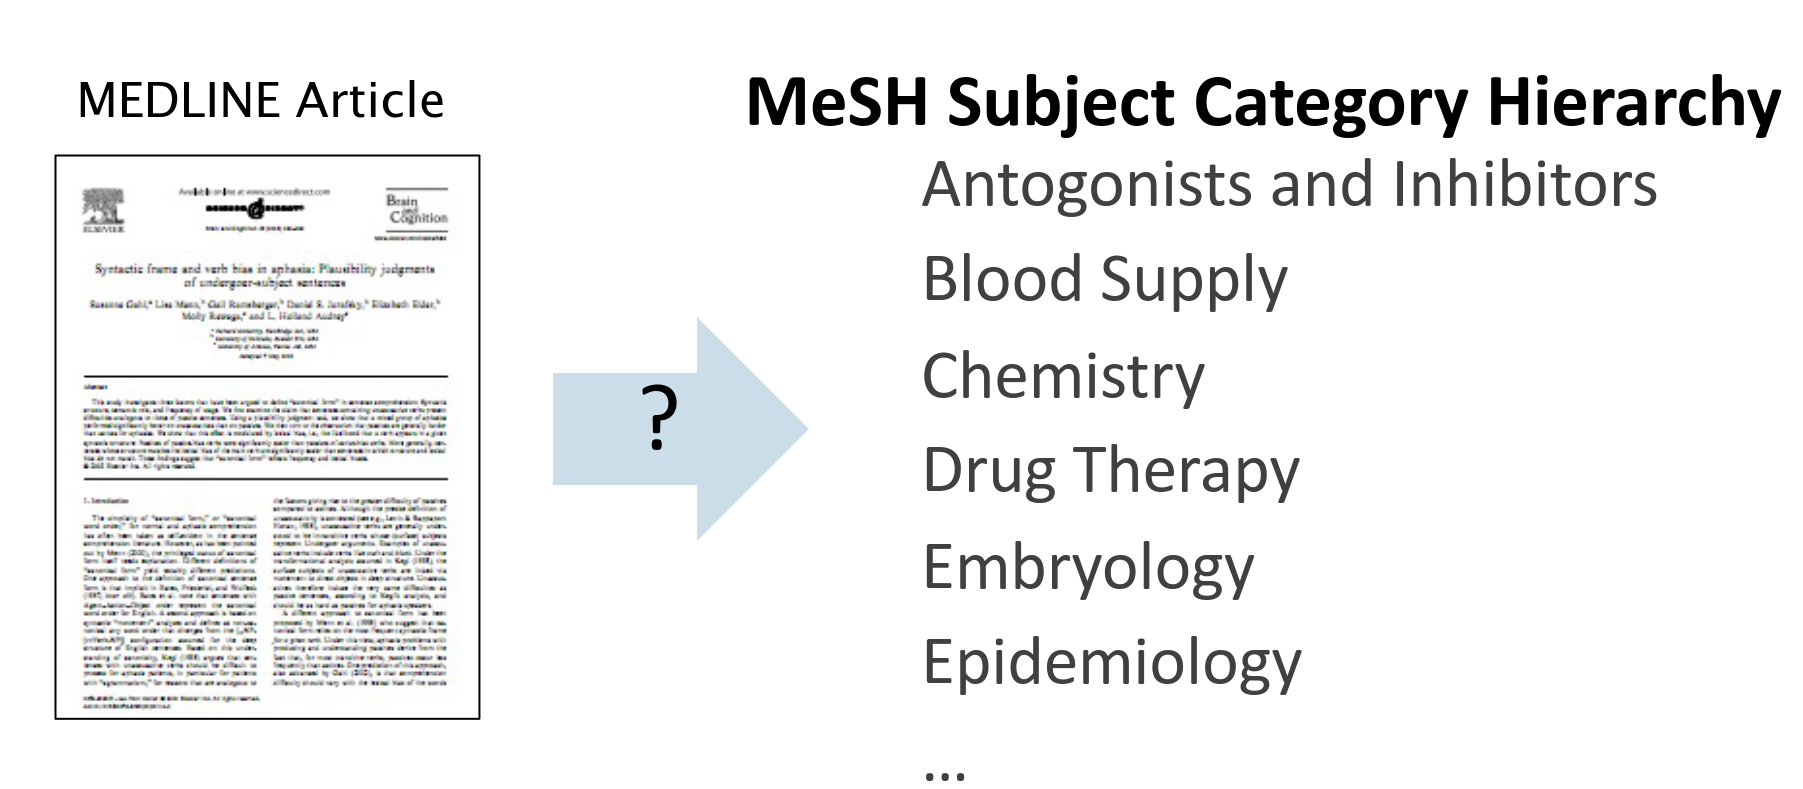
\includegraphics[scale = 0.2]{pics/medarticle.png}
    \caption{Ejemplo de clasificación por categorías clínicas.}
    \label{fig:medarticle}
\end{figure}



\end{example}



\begin{example}
Clasificación de sentimientos. La clasificación de sentimientos se utiliza para determinar si un documento exhibe un sentimiento positivo o negativo. Este enfoque se basa en el análisis del tono y las palabras utilizadas en el texto. A continuación, se presentan ejemplos de reseñas de películas y comentarios de restaurantes:

\begin{itemize}
    \item \textcolor{blue}{\textbf{+}} ...una película muy \textcolor{blue}{buena}, especialmente por los giros de la trama. ¡Fue \textcolor{blue}{espectacular}!
    \item \textcolor{red}{\textbf{-}} La actuación fue \textcolor{red}{patética}, destacando las escenas de baile como lo \textcolor{red}{peor}.
    \item \textcolor{blue}{\textbf{+}} ...la salsa de chocolate con almendras dulces es simplemente \textcolor{blue}{increíble} en este lugar. ¡Me \textcolor{blue}{encanta}!
    \item \textcolor{red}{\textbf{-}} ...la pizza estaba \textcolor{red}{horrible} y tenía un precio \textcolor{red}{ridículamente} alto.
\end{itemize}

Este enfoque se aplica en diversos casos, como medir la confianza del consumidor respecto a un producto o predecir resultados electorales y tendencias del mercado en función del sentimiento. Estas aplicaciones suelen ser el resultado de la implementación de modelos de análisis de sentimientos en datos procedentes de las redes sociales.
\end{example}




\section{Modelos Generativos}

Nuestra tarea principal consiste en aprender una función $f$ que asigne etiquetas $f(d)$ a las entradas $d$. El modelo Naïve Bayes sigue un enfoque probabilístico en el que buscamos estimar la probabilidad condicional $p(c|d)$ utilizando ejemplos de entrenamiento para todas las clases o etiquetas (por ejemplo, $c=c_1, c=c_2, \ldots, c=c_k$), donde $0 \leq p(c=c_j|d) \leq 1$ para cada $j$ y $\sum_j p(c=c_j|d)=1$. Luego, para cualquier entrada de prueba $\tilde{d}$, definimos $f(\tilde{d}) = c_{\text{MAP}} = \arg \max_c p(c|\tilde{d})$ como el estimador MAP (Maximum a Posteriori), lo cual equivale a seleccionar la clase más probable dada la información disponible en los datos.

Es importante señalar que existen dos enfoques principales en el aprendizaje automático en términos de la modelización de esta probabilidad condicional $p(c|d)$. Los modelos que intentan estimar $p(c|d)$ directamente de los datos se denominan modelos ``discriminativos'', como la regresión logística que exploraremos en el Capítulo~\ref{cap_lineales}.

Por otro lado, Naïve Bayes se clasifica como un ``modelo generativo''. Bajo este enfoque, se busca construir un modelo para cada clase y clasificar una entrada observando cuál clase tiene la mayor probabilidad de generar el ejemplo objetivo.

Este concepto puede formalizarse mediante el teorema de Bayes. Dado un documento $d$ y una clase $c$, tenemos:

\[
p(c | d) = \frac{p(d | c)p(c)}{p(d)}
\]

Aquí, $p(d | c)$ representa la ``verosimilitud'' que representa la probabilidad de que una clase particular ``genere'' el documento. Por otro lado, $p(c)$ se refiere a la probabilidad ``a priori'' de la clase y $p(d)$ corresponde a la probabilidad del documento, también conocida como ``evidencia''.

Dado que solo estamos interesados en encontrar la clase más probable para la clasificación, podemos eliminar el denominador, ya que se mantiene constante para todas las clases. Esto se expresa como:

\[
c_{\text{MAP}}  = \arg\max_{c} p(d | c)p(c)
\]

En resumen, el estimador MAP se utiliza para encontrar la clase más probable según la expresión anterior.

Alternativamente, podemos entender los modelos generativos como un intento de estimar la distribución conjunta $p(d, c)$ a partir de los ejemplos de entrenamiento. Utilizando la definición de probabilidad condicional, tenemos $p(d, c) = p(c)p(d|c)$, lo cual es equivalente al numerador que maximizamos previamente utilizando el teorema de Bayes.

\section{Naïve Bayes Multinomial}

Naïve Bayes, o el modelo Bayesiano ``ingenuo'' \cite{mccallum1998comparison}, se presenta como un modelo de clasificación generativo en el que un documento $d$ se representa como una bolsa de palabras $x_1, x_2, \ldots, x_n$. Similar al modelo vectorial explorado en el Capítulo~\ref{cap_ir}, en este modelo se omiten las posiciones de las palabras dentro del documento.

La verosimilitud del modelo probabilístico se expresa de la siguiente manera:

\[
p(d|c) = p(x_1, x_2, \ldots, x_n | c)
\]

Al estimar esta expresión sin hacer supuestos de independencia (es decir, contando las ocurrencias de $x_1, x_2, \ldots, x_n$ en cada clase), nos enfrentamos al mismo problema que se presenta en los modelos de lenguaje de n-gramas discutidos en el Capítulo~\ref{cap_plm}. A menos que tengamos un corpus infinitamente grande, este enfoque asignaría probabilidades nulas a las nuevas oraciones en las que se aplica el modelo, ya que es muy poco probable que éstas aparezcan en el corpus de entrenamiento.

Por lo tanto, recurrimos al supuesto de independencia condicional, que postula que las palabras son independientes entre sí cuando se condicionan a la clase. Esto nos permite factorizar la verosimilitud como el producto de factores individuales para cada palabra en el vocabulario:

\[
p(x_1, x_2, \ldots, x_n | c) = p(x_1 | c) \cdot p(x_2 | c) \cdot p(x_3 | c) \cdot \ldots \cdot p(x_n | c) = \prod_{i} p(x_i | c)
\]

Con esta factorización, la estimación MAP del modelo para clasificar un documento se formula de la siguiente manera:

\[
c_{\text{MAP}} = \arg\max_{c \in C} \prod_{i} p(x_i | c)p(c)
\]

\subsection{Estimación de parámetros}

Para estimar los parámetros del modelo Naive Bayes multinomial, se utiliza el método de estimación por máxima verosimilitud, asumiendo una distribución multinomial para $p(x_1, x_2, \ldots, x_n | c)$\footnote{Existe otra variante que asume una distribución Binomial pero no funciona tan bien para texto.}. Esto implica la creación de un ``mega-documento'' para cada clase $c_j$ mediante la concatenación de todos los documentos de esa clase. Luego, se calcula la frecuencia de todas las palabras $w_i$ del vocabulario en el mega-documento para cada clase $\text{count}(w_i, c_j)$.

La probabilidad estimada $\hat{p}(w_i | c_j)$ de la palabra $w_i$ dada la clase $c_j$ se obtiene dividiendo el conteo de ocurrencias de $w_i$ en el mega-documento de la clase $c_j$ por el total de palabras en el mega-documento:

\[
\hat{P}(w_i | c_j) = \frac{{\text{count}(w_i, c_j)}}{\sum_{w\in V}{\text{count}(w, c_j)}}
\]


La probabilidad previa de una clase $c_j$, $p(c_j)$, se estima de la siguiente manera:
    \[
    \hat{p}(c_j) = \frac{N_{c_j}}{N_{\text{total}}}
    \]
donde $N_{c_j}$ es el número de documentos en la clase $c_j$ y $N_{\text{total}}$ es el número total de documentos.


Una vez que el modelo Naïve Bayes (NB) ha sido entrenado, se puede emplear para clasificar un nuevo documento $\tilde{d}$ de la siguiente manera:

\[
c_{\text{NB}} = \arg\max_{c_j} p(c_j) \prod_{i \in \text{posiciones}} p(x_i | c_j)
\]

Básicamente, se debe iterar a través de las palabras en las posiciones del documento y calcular las probabilidades $p(c_j)$ y $p(x_i | c_j)$ para todas las clases y palabras del documento, para finalmente retornar la clase más probable. Estas probabilidades se derivan de los conteos almacenados durante el proceso de entrenamiento.

Cuando el documento de prueba $\tilde{d}$ contiene palabras que son desconocidas, es decir, no se encuentran en los datos de entrenamiento ni en el vocabulario, optamos por omitirlas. En este contexto, no asignamos ninguna probabilidad a estas palabras desconocidas durante el proceso de clasificación.

\subsection{Problemas al multiplicar muchas probabilidades}

La multiplicación de muchas probabilidades puede llevar a un underflow de punto flotante\footnote{\url{https://en.wikipedia.org/wiki/Arithmetic_underflow}}, especialmente cuando se manejan probabilidades pequeñas. Por ejemplo, $0.0006 \times 0.0007 \times 0.0009 \times 0.01 \times 0.5 \times 0.000008 \ldots$. Esto resulta en productos con valores nulos y clasificaciones erróneas.

Para abordar este problema, podemos recurrir a los logaritmos, ya que $\log(ab) = \log(a) + \log(b)$. En lugar de multiplicar las probabilidades, sumamos los logaritmos de las probabilidades. Así, el clasificador Naïve Bayes multinomial se puede expresar utilizando logaritmos de la siguiente manera:

\[
c_{\text{NB}} = \arg\max_{c_j \in C} \left(\log(P(c_j)) + \sum_{i \in \text{posiciones}} \log(P(x_i | c_j))\right)
\]

La función logaritmo es monótona creciente, lo que significa que si una probabilidad es mayor que otra, el logaritmo de esa probabilidad también será mayor que el logaritmo de la otra probabilidad. Esto preserva el orden relativo de las probabilidades, por lo que el resultado óptimo de la clasificación no se ve afectado.

Al aplicar logaritmos, el clasificador Naive Bayes se convierte en un modelo lineal (Capítulo~\ref{cap_lineales}), donde la predicción es el argmax de la suma de los logaritmos de las probabilidades y las entradas (logaritmos de las probabilidades condicionales). En otras palabras, Naive Bayes se convierte en un clasificador lineal que opera en el espacio logarítmico.

\subsection{Suavizamiento de Laplace}

De forma similar a los modelos de lenguaje de n-gramas mencionados en el Capítulo~\ref{cap_plm}, Naïve Bayes también enfrenta problemas de probabilidades nulas.

Supongamos que estamos trabajando en un problema de clasificación de sentimientos con clases positivo y negativo. Por alguna razón, la palabra ``fantástico'' no aparece en ningún documento negativo. Luego, imaginemos que queremos clasificar el documento $\tilde{d}=$ ``Qué fantástico, acabo de aburrirme como nunca viendo la peor película de mi vida''. Claramente, este documento es negativo, pero si usamos la estimación de máxima verosimilitud, la probabilidad $\hat{p}(\text{``fantástico''} \mid \text{negativo})$ sería:

\[
\hat{p}(\text{``fantástico''} \mid \text{negativo}) = \frac{\text{count}(\text{``fantástico''}, \text{negativo})}{\sum_{w \in V} \text{count}(w, \text{negativo})} = \frac{0}{\sum_{w \in V} \text{count}(w, \text{positivo})} = 0
\]

El problema es que esta probabilidad cero anularía toda la evidencia proporcionada por otras palabras muy indicativas de la clase negativa, como ``aburrirme'' y ``peor'' por la forma multiplicativa de la función de verosimilitud del modelo, y el clasificador Naïve Bayes terminaría clasificando el ejemplo en la clase ``positiva''.

Para abordar este problema, podemos utilizar la técnica de suavizamiento de Laplace, que consiste en agregar un conteo adicional a todas las combinaciones de palabras y clases y ajustar el denominador con el tamaño del vocabulario $V$ para garantizar una normalización adecuada. La estimación suavizada $\hat{p}(w_i \mid c)$ queda de la siguiente manera:

\[
\hat{p}(w_i \mid c) = \frac{\text{count}(w_i, c) + 1}{\sum_{w \in V} (\text{count}(w, c) + 1)} = \frac{\text{count}(w_i, c) + 1}{(\sum_{w \in V} \text{count}(w, c))+|V|}
\]

Esta técnica aborda el problema de las probabilidades nulas, ya que ahora cualquier palabra del vocabulario, incluso si nunca se ha visto con alguna clase, recibirá una probabilidad condicional mayor a cero. Como pueden ver, esta técnica permite que cierta masa de probabilidad se distribuya a palabras no vistas de manera similar a  las técnicas de descuento vistas en el Capítulo de modelos de lenguaje (Capítulo~\ref{cap_plm}).


\begin{example}

Supongamos que tenemos el conjunto de entrenamiento mostrado en la Tabla~\ref{tab_nb_train} y queremos clasificar el ejemplo de la Tabla~\ref{tab_nb_test}.


\begin{table}[h]
\centering
\begin{tabular}{|c|p{0.7\textwidth}|}
\hline
\textbf{Categoría} & \textbf{Texto} \\
\hline
Perú & Lima Lima Trujillo \\
\hline
Chile & Santiago Concepción Concepción\\
\hline
Perú & Perú Lima Trujillo América\\
\hline
Chile & Chile América Santiago \\
\hline
\end{tabular}
\caption{Datos de Entrenamiento.}
\label{tab_nb_train}
\end{table}




\begin{table}[h]
\centering
\begin{tabular}{|c|p{0.7\textwidth}|}
\hline
\textbf{Categoría} & \textbf{Texto} \\
\hline
? & América Lima Perú Santiago \\
\hline
\end{tabular}
\caption{Ejemplo de Prueba.}
\label{tab_nb_test}
\end{table}

En este ejemplo, $|V|=7$, y tenemos dos clases: $c_1=$ Perú y $c_2=$ Chile.

La Tabla~\ref{tab_nb_conteos} muestra los conteos calculados a partir de los datos de entrenamiento.

\begin{table}[h]
\centering
\begin{tabular}{|c|c|c|c|}
\hline
id\_palabra & palabra & count($w_i$,Perú) & count($w_i$,Chile) \\
\hline
$w_1$ & América & 1 & 1 \\
$w_2$ & Chile & 0 & 1 \\
$w_3$ & Concepción & 0 & 2 \\
$w_4$ & Lima & 3 & 0 \\
$w_5$ & Perú & 1 & 0 \\
$w_6$ & Santiago & 0 & 2 \\
$w_7$ & Trujillo & 2 & 0 \\
\hline
\end{tabular}
\caption{Tabla de Conteos.}
\label{tab_nb_conteos}
\end{table}

Ahora, debemos calcular las probabilidades condicionales suavizadas:
\[
\hat{p}(w_i \mid c) = \frac{\text{count}(w_i, c) + 1}{\left(\sum_{w \in V} \text{count}(w, c)\right) + |V|}
\]
para todas las palabras y clases\footnote{Alternativamente podríamos sumar los logartimos de las probabilidades.}.

El denominador de esta expresión para cada clase corresponde al largo del ``mega-documento'' que junta todos los documentos de la misma clase más el tamaño del vocabulario, que sería $7+7=14$ para Perú y $6+7=13$ para Chile.

Las probabilidades resultantes se muestran en la Tabla~\ref{tab_nb_probs}.

\begin{table}[h]
\centering
\begin{tabular}{|c|c|c|c|}
\hline
id\_palabra & palabra & $\hat{p}(w_i \mid c=\text{Perú})$ & $\hat{p}(w_i \mid c=\text{Chile})$ \\
\hline
$w_1$ & América & $\frac{1+1}{14}=0.14$ & $\frac{1+1}{13}=0.15$ \\
$w_2$ & Chile & $\frac{0+1}{14}=0.07$ & $\frac{1+1}{13}=0.15$ \\
$w_3$ & Concepción & $\frac{0+1}{14}=0.07$ & $\frac{2+1}{13}=0.23$ \\
$w_4$ & Lima & $\frac{3+1}{14}=0.29$ & $\frac{0+1}{13}=0.08$ \\
$w_5$ & Perú & $\frac{1+1}{14}=0.14$ & $\frac{0+1}{13}=0.08$ \\
$w_6$ & Santiago & $\frac{0+1}{14}=0.07$ & $\frac{2+1}{13}=0.23$ \\
$w_7$ & Trujillo & $\frac{2+1}{14}=0.21$ & $\frac{0+1}{13}=0.08$ \\
\hline
\end{tabular}
\caption{Probabilidades condicionales suavizadas.}
\label{tab_nb_probs}
\end{table}

Ahora necesitamos estimar la probabilidad a priori de cada clase:
    \[
    \hat{p}(c_j) = \frac{N_{c_j}}{N_{\text{total}}}
    \]

Ambas clases ocurren en 2 documentos sobre un total de 4. Entonces, $\hat{p}(c=\text{Perú})=0.5$ y $\hat{p}(c=\text{Chile})=0.5$.

Ahora debemos calcular:
\[
c_{\text{NB}} = \arg\max_{c_j} p(c_j) \prod_{i \in \text{posiciones}} p(x_i | c_j)
\]

Esto implica iterar posiciones para ambas clases del documento de prueba:

\[
c_{\text{Perú}} = 0.14\times 0.29\times 0.14\times 0.07\times 0.5=0.00019894
\]

\[
c_{\text{Chile}} = 0.15\times 0.08\times 0.08\times 0.23\times 0.5=0.0001104
\]
Entonces, $c_{\text{NB}}=$``Perú'' y clasificamos el documento a la clase ``Perú''.
\end{example}



\subsection{Naïve Bayes como modelo de lenguaje}

A continuación, exploraremos una interpretación del modelo Naïve Bayes utilizando conceptos de modelos de lenguaje. El supuesto de independencia condicional de palabras en Naïve Bayes lo asemeja mucho a un modelo de lenguaje de unigramas que se discutió en el Capítulo~\ref{cap_plm}.

Específicamente, la función de verosimilitud en el modelo Naïve Bayes multinomial se puede entender como la construcción de un modelo de lenguaje de unigramas para cada clase.

\begin{example}
Por ejemplo, consideremos un problema de clasificación de sentimientos con las clases ``positivo'' y ``negativo'' y los siguientes parámetros del modelo:

\begin{center}
\begin{tabular}{|ccc|} \hline
\textbf{Palabra} & $p(w|c=\text{``positivo''})$ & $p(w|c=\text{``negativo''})$  \\ \hline
Yo & 0.1 & 0.2 \\
amé & 0.1 & 0.001 \\
esta & 0.01 & 0.01 \\
gran & 0.05 & 0.005 \\
película & 0.1 & 0.1 \\
... & ... & ... \\ \hline
\end{tabular}
\end{center}

Cada una de las dos columnas anteriores se puede interpretar tanto como las probabilidades condicionales del modelo Naïve Bayes como las probabilidades de dos modelos de lenguaje de unigramas construidos con los datos de entrenamiento de cada clase. Para ilustrar esto, supongamos que deseamos clasificar la oración $d=$ ``Yo amé esta gran película''. Podemos calcular:

\[p(d|\text{``positivo''}) = 0.1 \times 0.1 \times 0.01 \times 0.05 \times 0.1 = 0.0000005\]
\[p(d|\text{``negativo''}) = 0.2 \times 0.001 \times 0.01 \times 0.005 \times 0.1 = 0.0000000010\]

Observamos que el modelo positivo asigna una probabilidad más alta a la oración:
\[p(d|\text{''positivo''}) > p(d|\text{''negativo''})\]

Este cálculo puede interpretarse indistintamente como la probabilidad asignada por cada modelo de lenguaje a la oración objetivo o como el resultado de la función de verosimilitud del modelo Naïve Bayes.
\end{example}

Es importante destacar que en este análisis estamos utilizando solo la parte de verosimilitud del modelo Naïve Bayes. Una vez que multiplicamos por la probabilidad a priori de las clases en Naïve Bayes, podríamos obtener resultados diferentes a los obtenidos con el modelo de lenguaje.



\section{Evaluación}

La evaluación juega un papel crucial en la construcción de sistemas de PLN basados en aprendizaje automático. Al construir estos sistemas, es común llevar a cabo comparaciones y experimentos con diversos modelos durante el proceso de entrenamiento, con el fin de elegir el modelo más idóneo para su posterior implementación en producción. Generalmente, adoptamos un enfoque cuantitativo para evaluar modelos, contrastando las predicciones realizadas con las predicciones esperadas, y resumiendo estos resultados mediante métricas de evaluación. Este enfoque cuantitativo se prefiere debido a que un enfoque cualitativo o de inspección manual no resulta escalable. Ilustremos este proceso de evaluación con un ejemplo.


\begin{example}
Supongamos un problema de clasificación binaria, para la cual queremos comparar dos modelos de clasificación $m_1$ y $m_2$. Probamos los modelos sobre un conjunto de datos de prueba y obtenemos las predicciones señaladas en la Tabla~\ref{tab:ej_sentimiento}.

\begin{table}[htbp]
\centering
\begin{tabular}{|l|l|l|l|}
\hline
\textbf{Texto} & \textbf{Clase} & \textbf{m1} & \textbf{m2} \\
\hline
no estoy bien & negativo & negativo & positivo \\
al fin! & positivo & positivo & negativo \\
que pena & negativo & negativo & negativo \\
feliz & positivo & positivo & positivo \\
no quiero & negativo & positivo & negativo \\
jamás! & negativo & negativo & negativo \\
buena idea & positivo & positivo & negativo \\
chao contigo & negativo & positivo & negativo \\
\hline
\end{tabular}
\caption{Sentimiento de texto}
\label{tab:ej_sentimiento}
\end{table}

Se puede observar que tanto el modelo $m_1$ como el modelo $m_2$ presentan errores en sus predicciones al compararse con las categorías reales de los ejemplos (columna clase), también conocidas como ``gold labels'' o ``ground truth''. Sin embargo, ¿cómo determinamos cuál modelo es mejor? Para abordar esta pregunta, resulta conveniente calcular métricas de desempeño, las cuales se derivan al contrastar las predicciones de un modelo con sus salidas esperadas.
\end{example}

\subsection{Matriz de Confusión}

La mayoría de las métricas de evaluación para problemas de clasificación se derivan de una matriz de confusión (véase Tabla~\ref{tab:matriz_confusion}), la cual representa una tabla de contingencia entre las predicciones de un modelo y las salidas esperadas en un conjunto de prueba. Para problemas de clasificación binaria, esta matriz consta de 4 componentes:

\begin{enumerate}
\item Verdadero Positivo (VP): cuando el modelo predice correctamente la clase positiva, coincidiendo con la salida esperada.
\item Verdadero Negativo (VN): cuando el modelo predice correctamente la clase negativa, coincidiendo con la salida esperada.
\item Falso Negativo (FN): cuando el modelo predice incorrectamente la clase negativa, siendo la salida esperada positiva.
\item Falso Positivo (FP): cuando el modelo predice incorrectamente la clase positiva, siendo la salida esperada negativa.
\end{enumerate}

Es importante destacar que la definición de qué constituye la clase positiva es arbitraria en un problema de clasificación; generalmente se refiere a la clase que se desea detectar. En el caso de la clasificación de sentimientos, es una coincidencia que la clase positiva se asocie con el sentimiento ``positivo''. Esta consideración es fundamental, ya que el valor de algunas métricas de desempeño (como precisión, recall y $F_1$) depende de la elección de la clase positiva.

\begin{table}[htbp]
\centering
\begin{tabular}{|c|c|c|}
\hline
\textbf{} & \textbf{Modelo Positivo} & \textbf{Modelo Negativo} \\
\hline
\textbf{Real Positivo} & Verdadero Positivo (VP) & Falso Negativo (FN) \\
\hline
\textbf{Real Negativo} & Falso Positivo (FP) & Verdadero Negativo (VN) \\
\hline
\end{tabular}
\caption{Matriz de confusión}
\label{tab:matriz_confusion}
\end{table}


\subsection{Métricas de Desempeño}

\textbf{Recall} (exhaustividad) (también conocido como \textbf{Sensibilidad} o \textbf{Tasa de Verdaderos Positivos}):
\[ \text{Recall} = \frac{VP}{VP + FN} \]

\textbf{Precisión}:
\[ \text{Precisión} = \frac{VP}{VP + FP} \]

\textbf{Accuracy} (exactitud):
\[ \text{Accuracy} = \frac{VP + VN}{VP + FP + VN + FN} \]


¿Por qué no usamos la exactitud como nuestra métrica?

Imagina que vimos 1 millón de tweets:
\begin{itemize}
\item 100 de ellos hablaban sobre Delicious Pie Co.
\item 999,900 hablaban de otra cosa.
\end{itemize}

Podríamos construir un clasificador tonto que simplemente etiquete todos los tweets como "no sobre pasteles":
\begin{itemize}
\item ¡¡¡Obtendría una exactitud del 99.99\%!!! ¡¡¡Wow!!!
\item ¡Pero sería inútil! ¡No devuelve los comentarios que estamos buscando!
\end{itemize}

Por eso usamos precisión y recall en su lugar.


\textbf{Precisión} mide el porcentaje de elementos que el sistema detectó (es decir, los elementos que el sistema etiquetó como positivos) que son realmente positivos (según las etiquetas de oro humanas).

\[
\text{Precisión} = \frac{\text{Verdaderos Positivos}}{\text{Verdaderos Positivos + Falsos Positivos}}
\]

\textbf{Recall} mide el porcentaje de elementos que el sistema identificó correctamente de todos los elementos que deberían haber sido identificados.

\[
\text{Recall} = \frac{\text{Verdaderos Positivos}}{\text{Verdaderos Positivos + Falsos Negativos}}
\]


Considera nuestro clasificador tonto de pasteles que simplemente etiqueta nada como "sobre pasteles".

\begin{itemize}
  \item Exactitud = 99.99\% (etiqueta correctamente la mayoría de los tweets como no relacionados con pasteles)
  \item Recall = 0 (no detecta ninguno de los 100 tweets relacionados con pasteles)
\end{itemize}

La precisión y el recall, a diferencia de la exactitud, enfatizan los verdaderos positivos:
\begin{itemize}
  \item Se centran en encontrar las cosas que se supone que debemos buscar.
\end{itemize}

\subsection{Una Medida Combinada: Medida F}
La medida F es un número único que combina la precisión (P) y el recall (R), definida como:
\[
F_\beta = \frac{(\beta^2+1)PR}{\beta^2P + R}
\]

La medida F, definida con el parámetro $\beta$, pondera diferencialmente la importancia del recall y la precisión.
\begin{itemize}
  \item $\beta > 1$ favorece al recall
  \item $\beta < 1$ favorece a la precisión
\end{itemize}

Cuando $\beta = 1$, la precisión y el recall son iguales, y tenemos la medida $F_1$ equilibrada:
\[
F_1 = \frac{2PR}{P + R}
\]

\subsection{Conjuntos de Prueba de Desarrollo ("Devsets")}

\begin{itemize}
 \item Para evitar el sobreajuste y proporcionar una estimación más conservadora del rendimiento, comúnmente utilizamos un enfoque de tres conjuntos: conjunto de entrenamiento, conjunto de desarrollo y conjunto de prueba.
\begin{figure}[h]
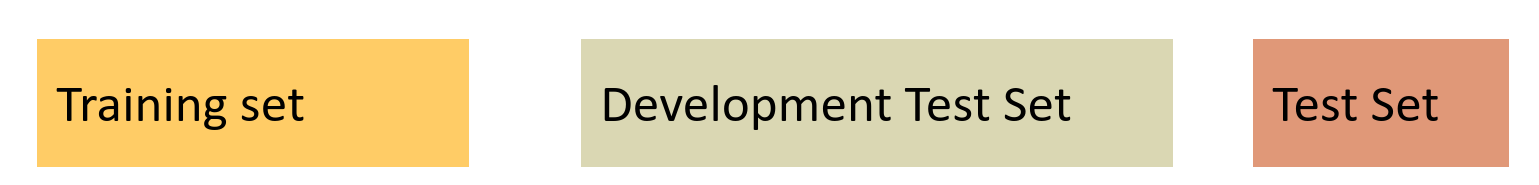
\includegraphics[scale = 0.23]{pics/devsets.png}
\end{figure}

\begin{itemize}
\item \textbf{Conjunto de entrenamiento}: Se utiliza para entrenar el modelo.
\item \textbf{Conjunto de desarrollo}: Se utiliza para ajustar el modelo y seleccionar los mejores hiperparámetros.
\item \textbf{Conjunto de prueba}: Se utiliza para informar el rendimiento final del modelo.
\end{itemize}

\item Este enfoque garantiza que el modelo no esté ajustado específicamente al conjunto de prueba, evitando el sobreajuste.
\item Sin embargo, crea una paradoja: queremos la mayor cantidad de datos posible para el entrenamiento, pero también para el conjunto de desarrollo.
\item ¿Cómo dividimos los datos?

\end{itemize}





\subsection{Validación Cruzada: Múltiples Divisiones}

La validación cruzada nos permite utilizar todos nuestros datos para el entrenamiento y la prueba sin tener un conjunto de entrenamiento, conjunto de desarrollo y conjunto de prueba fijos.  Elegimos un número $k$ y dividimos nuestros datos en $k$ subconjuntos disjuntos llamados pliegues.  En cada iteración, uno de los pliegues se selecciona como conjunto de prueba mientras que los $k-1$ pliegues restantes se utilizan para entrenar el clasificador.

Calculamos la tasa de error en el conjunto de prueba y repetimos este proceso $k$ veces.  Finalmente, promediamos las tasas de error de estas $k$ ejecuciones para obtener una tasa de error promedio.

Por ejemplo, la validación cruzada de 10 pliegues implica entrenar 10 modelos con el 90\% de los datos y probar cada modelo por separado.  Las tasas de error resultantes se promedian para obtener la estimación final del rendimiento. Sin embargo, la validación cruzada requiere que todo el corpus sea ciego, lo que impide examinar los datos para sugerir características o comprender el comportamiento del sistema.  Para abordar esto, se crea un conjunto de entrenamiento y un conjunto de prueba fijos, y se realiza la validación cruzada de 10 pliegues dentro del conjunto de entrenamiento.  La tasa de error se calcula convencionalmente en el conjunto de prueba.


\begin{center}
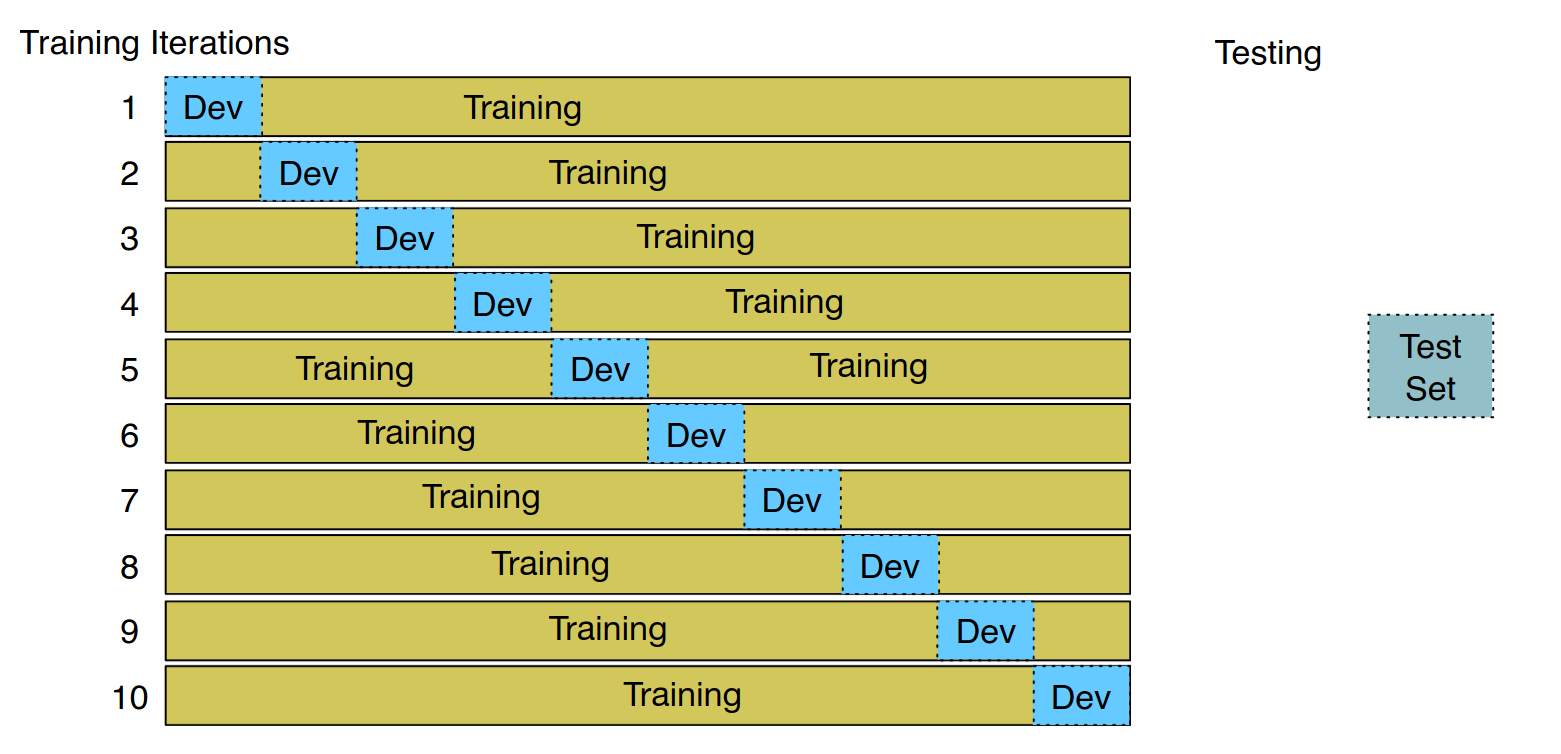
\includegraphics[scale=0.28]{pics/cv.png}
\end{center}

\section{Conjuntos de entrenamiento, prueba y validación}
Cuando entrenamos un modelo, nuestro objetivo es producir una función $f(\vec{x})$ que mapee correctamente las entradas $\vec{x}$ a las salidas $\hat{y}$ según lo evidenciado por el conjunto de entrenamiento. La evaluación del rendimiento en los datos de entrenamiento puede ser engañosa, ya que nuestro objetivo es entrenar una función capaz de generalizar a ejemplos no vistos. Una forma común de abordar esto es dividir el conjunto de entrenamiento en subconjuntos de entrenamiento y prueba (80\% y 20\% respectivamente). Se entrena el modelo en el subconjunto de entrenamiento y se calcula la precisión en el subconjunto de prueba.

Sin embargo, este enfoque tiene una limitación. En la práctica, a menudo se entrenan varios modelos, se comparan sus calidades y se selecciona el mejor. Si se selecciona el mejor modelo en función de la precisión en el subconjunto de prueba, se obtendrá una estimación excesivamente optimista de la calidad del modelo. No se sabe si la configuración elegida del clasificador final es buena en general o simplemente es buena para los ejemplos particulares en los subconjuntos de prueba.

La metodología aceptada es utilizar una división de tres vías de los datos en conjuntos de entrenamiento, validación (también llamado desarrollo) y prueba\footnote{Un enfoque alternativo es la validación cruzada, pero no se escala bien para entrenar redes neuronales profundas.}. Esto proporciona dos conjuntos apartados: un conjunto de validación (también llamado conjunto de desarrollo) y un conjunto de prueba. Todos los experimentos, ajustes, análisis de errores y selección de modelos deben realizarse

basados en el conjunto de validación. Luego, una única ejecución del modelo final sobre el conjunto de prueba proporcionará una buena estimación de su calidad esperada en ejemplos no vistos. Es importante mantener el conjunto de prueba lo más limpio posible, realizando la menor cantidad de experimentos posible en él. Incluso algunos defienden que no se deben mirar siquiera los ejemplos en el conjunto de prueba, para evitar sesgar el diseño del modelo.

\begin{figure}[htb]
	\centering
	 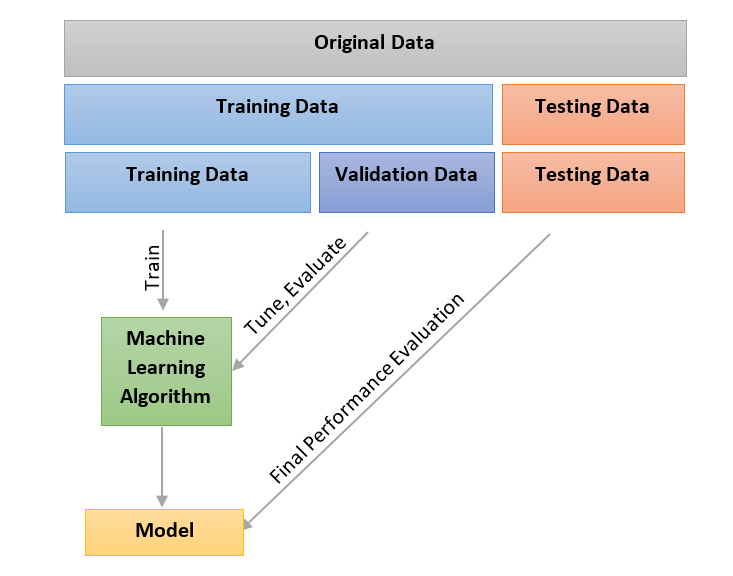
\includegraphics[scale=0.55]{pics/validation.png}
\end{figure}

\footnotetext{Fuente: \url{https://www.codeproject.com/KB/AI/1146582/validation.PNG}}


\subsection{Matriz de Confusión para clasificación de 3 clases}


\begin{center}
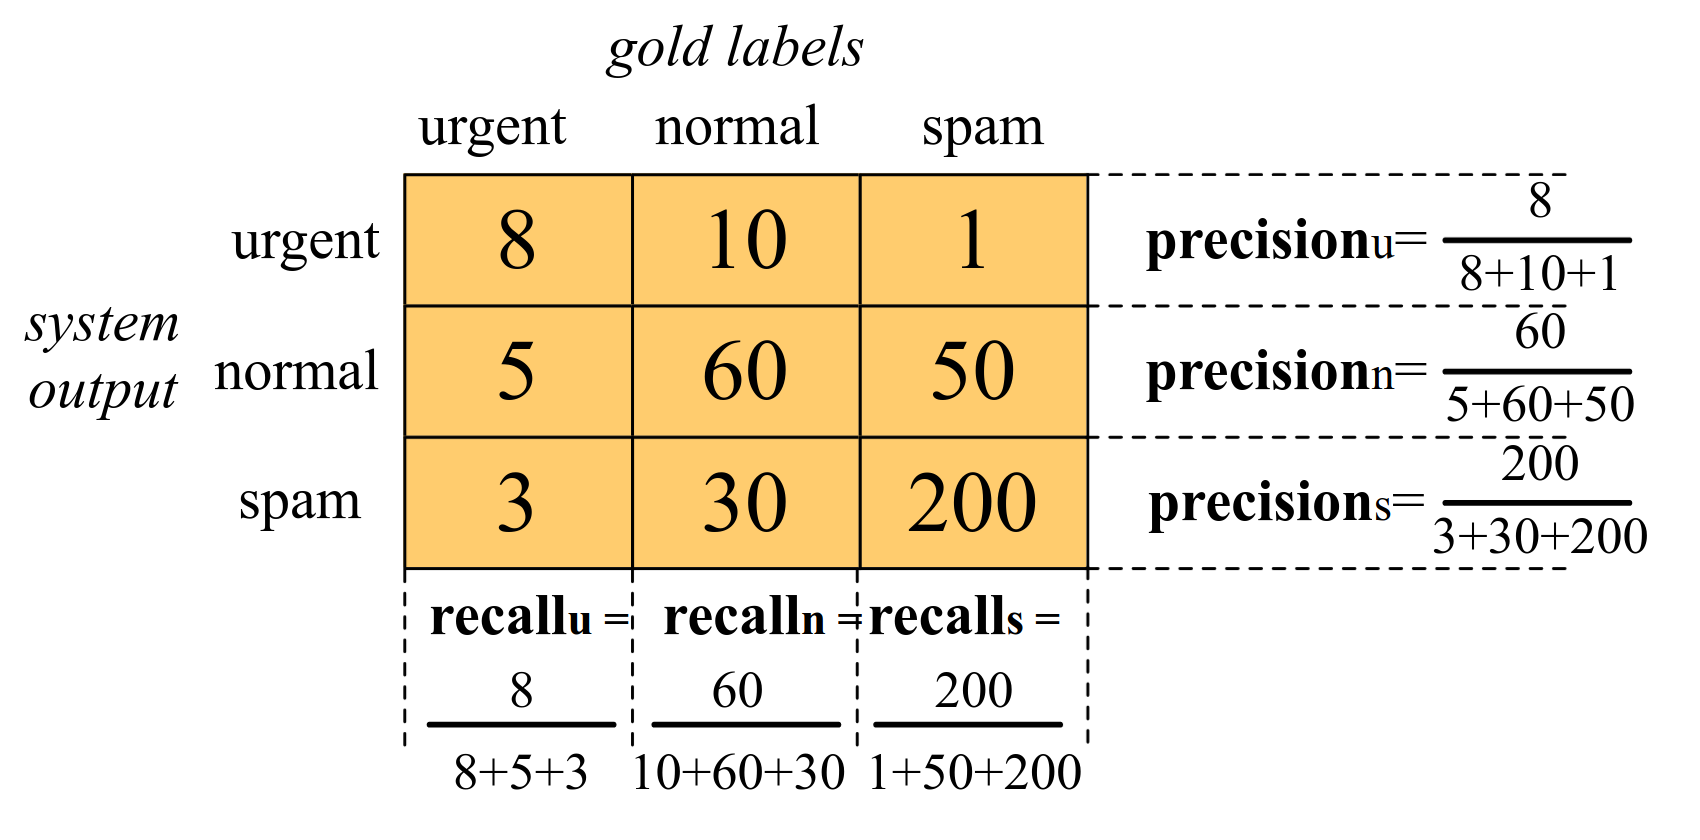
\includegraphics[scale=0.23]{pics/confmatrix.png}
\end{center}

Cómo combinar métricas binarias (Precisión, Recall, $F_1$) de más de 2 clases para obtener una métrica única:
\begin{itemize}
 \item Macro-promedio:
 \begin{itemize}
    \item Calcular las métricas de rendimiento (Precisión, Recall, $F_1$) para cada clase individualmente.
    \item Promediar las métricas en todas las clases.
 \end{itemize}
 \item Micro-promedio:
 \begin{itemize}
    \item Recopilar las decisiones para todas las clases en una matriz de confusión.
    \item Calcular la Precisión y el Recall a partir de la matriz de confusión.
 \end{itemize}
\end{itemize}

\begin{center}
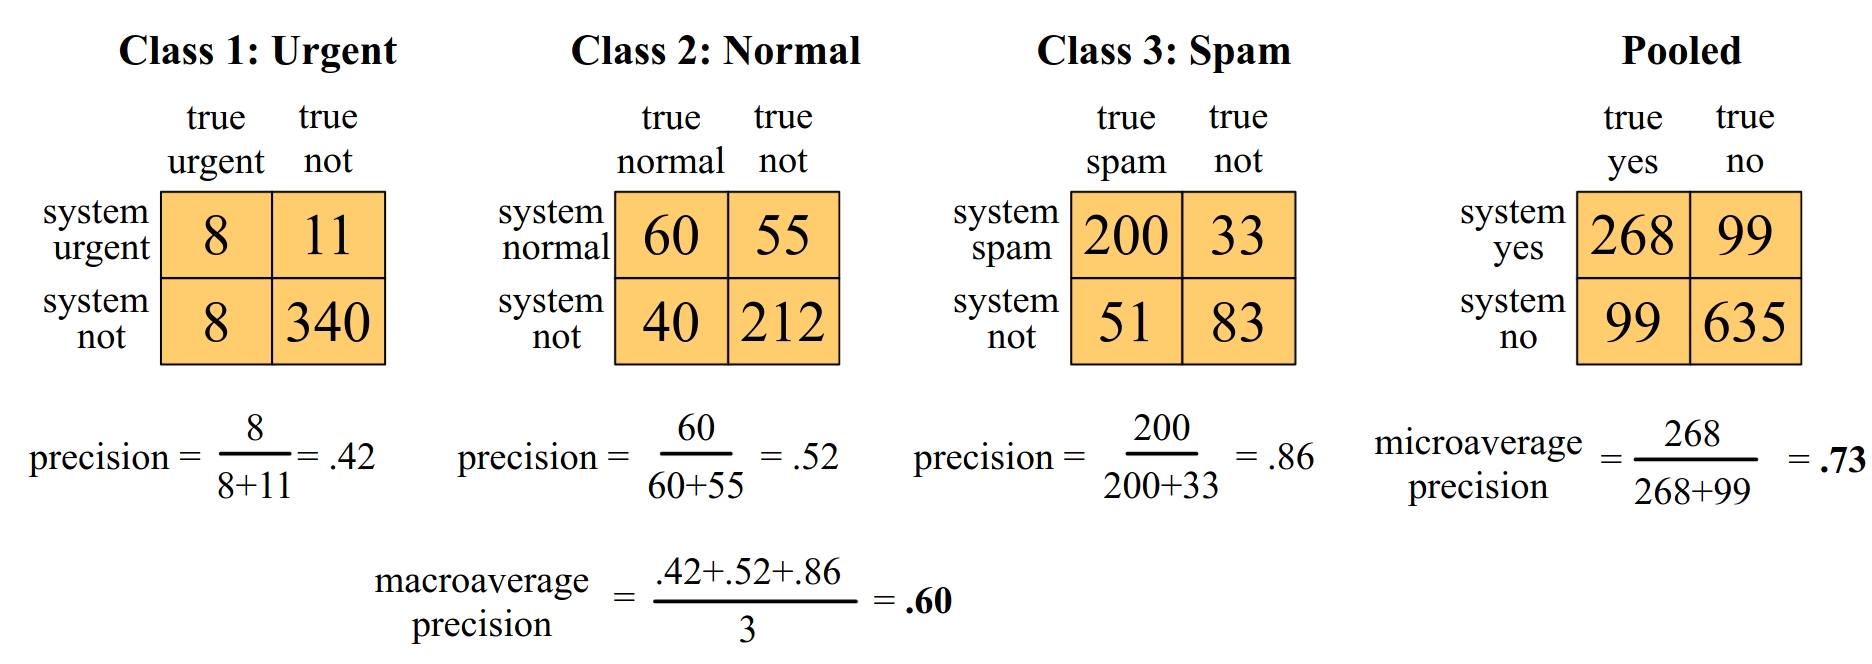
\includegraphics[scale=0.23]{pics/confmatrixmulti.png}
\end{center}
